\section{Thảo luận}
\label{sec:discussion}

\subsection{Độ chính xác, thời gian và khả năng giải thích}
Bốn mô hình nằm trên một đường đánh đổi khá rõ giữa độ chính xác, chi phí và độ dễ đọc (\cref{tab:accuracy,tab:time}).

\textbf{Naïve Bayes} (\accTestNB\%) rẻ nhất: huấn luyện trong \fitNB\,s, vì chỉ cần trung bình và phương sai từng pixel theo lớp. Nhưng giả thiết các pixel độc lập có điều kiện theo lớp sai với ảnh chữ số, nơi các pixel lân cận tương quan mạnh. Hệ quả thấy rõ ở bước chọn siêu tham số: với \texttt{var\_smoothing} mặc định $10^{-9}$ validation chỉ đạt khoảng 56\%, và tăng lên $0.1$ mới đạt \accValNB\%. Giải thích hợp lý (chúng tôi chưa kiểm chứng riêng): nhiều pixel ở rìa ảnh gần như luôn bằng 0 nên phương sai ước lượng rất nhỏ, và một pixel hiếm khi sáng lên cũng đủ kéo log-likelihood của lớp đó xuống rất thấp; làm trơn phương sai bù lại điều này. Đổi lại, mô hình dễ giải thích nhất: ảnh trung bình của từng lớp (\cref{fig:interp}, hàng đầu) cho biết nó ``nhìn thấy'' gì.

\textbf{Softmax} (\accTestSM\%) là mô hình tuyến tính: mỗi lớp là một mẫu (template) $w_k$ và lớp nào có điểm $w_k^\top x+b_k$ cao nhất thì thắng. Nó nhanh (\fitSM\,s huấn luyện, \latSM\,ms mỗi ảnh) nhưng bị giới hạn bởi biên quyết định tuyến tính. Trọng số (\cref{fig:interp}, hàng hai) đọc được ở mức mờ: có vệt dương/âm theo nét của chữ số, song nhiễu hơn ảnh trung bình của Naïve Bayes.

\textbf{MLP} (\accTestMLP\%) là mô hình tốt nhất và vẫn rẻ: \fitMLP\,s huấn luyện vì dừng sớm ở epoch 14 (khôi phục epoch 9). Đổi lại, các đơn vị lớp ẩn (\cref{fig:interp}, hàng ba) gần như không đọc được bằng mắt. Chênh lệch giữa train (\accTrainMLP\%) và test (\accTestMLP\%) khoảng \gapMLP{} điểm phần trăm; dropout không giúp thêm ở lượt quét (khoảng \texttt{p\_drop}=0.2 chỉ sát giá trị 0, trong phạm vi nhiễu).

\textbf{AdaBoost} (\accTestADA\%) đạt độ chính xác cao nhưng đắt nhất mọi mặt: \fitADA\,s huấn luyện, \predADA\,s cho $10\,000$ ảnh test, \latADA\,ms cho một ảnh vì phải duyệt $393$ cây, và tệp xuất ra nặng hơn $15$\,MiB. Độ chính xác train đạt \accTrainADA\% từ rất sớm (\cref{fig:curves}c) trong khi validation vẫn tăng chậm theo số vòng; đây là hành vi quen thuộc của boosting với cây sâu: sai số huấn luyện về 0 không có nghĩa là hết khả năng tổng quát hóa. Mô hình có một dạng giải thích riêng: tần suất các pixel được dùng để chia nhánh (\cref{fig:interp}, hàng cuối) tập trung ở vùng trung tâm, nơi có nét chữ. Điểm số của nó là tỉ lệ phiếu, \emph{chưa hiệu chỉnh} thành xác suất.

\begin{figure}[H]
\centering
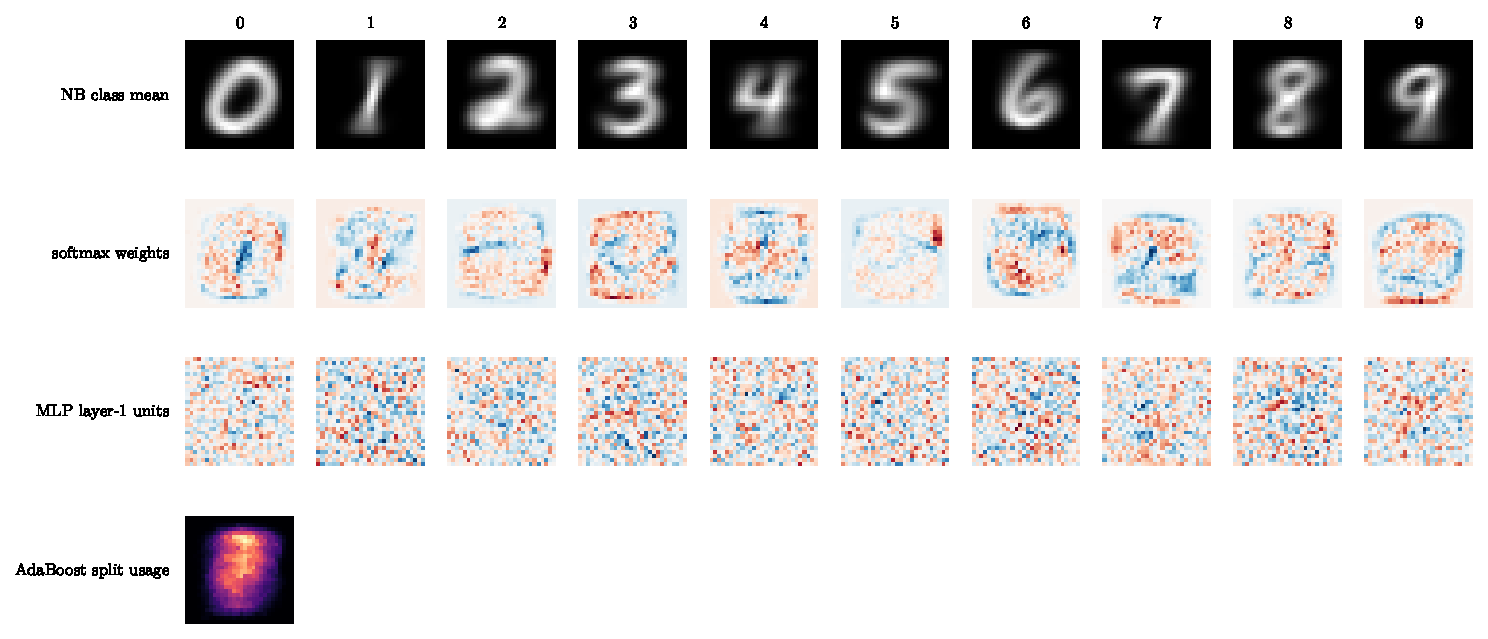
\includegraphics[width=\textwidth]{../results/figures/interpretability.pdf}
\caption{Cái mà mỗi mô hình ``học'': ảnh trung bình theo lớp của Naïve Bayes, trọng số softmax (đỏ dương, xanh âm), một số đơn vị ẩn đầu tiên của MLP và bản đồ tần suất chia nhánh của AdaBoost.}
\label{fig:interp}
\end{figure}

\subsection{Những chữ số bị nhầm}
Cặp nhầm nhiều nhất của từng mô hình (nhãn thật$\to$nhãn dự đoán, số ảnh) trong tập test:
\begin{description}[leftmargin=0pt,labelindent=0pt,style=unboxed,itemsep=2pt]
\item[Gaussian NB.] 4$\to$9 (284), 5$\to$3 (97), 7$\to$9 (91).
\item[Softmax regression.] 4$\to$9 (39), 5$\to$3 (36), 2$\to$8 (35).
\item[MLP.] 7$\to$9 (8), 9$\to$4 (7), 5$\to$3 (7).
\item[AdaBoost-SAMME.] 5$\to$3 (12), 4$\to$9 (12), 7$\to$9 (10).
\end{description}

Cả bốn mô hình đều nhầm $4\to9$ hoặc $7\to9$ và $5\to3$: những cặp có nét chung (đầu chữ 4 và chữ 9 khép hay hở, nét ngang của 7). Với Naïve Bayes riêng cặp $4\to9$ chiếm tới 284 trong \errorsNB{} lỗi. Với MLP, chỉ \errorsMLP{} ảnh sai, và một số ảnh sai là những chữ khó đọc ngay cả với người (\cref{fig:errors}); nên một phần lỗi còn lại có thể đến từ chính nhãn và nét chữ mơ hồ chứ không chỉ từ mô hình.

\begin{figure}[H]
\centering
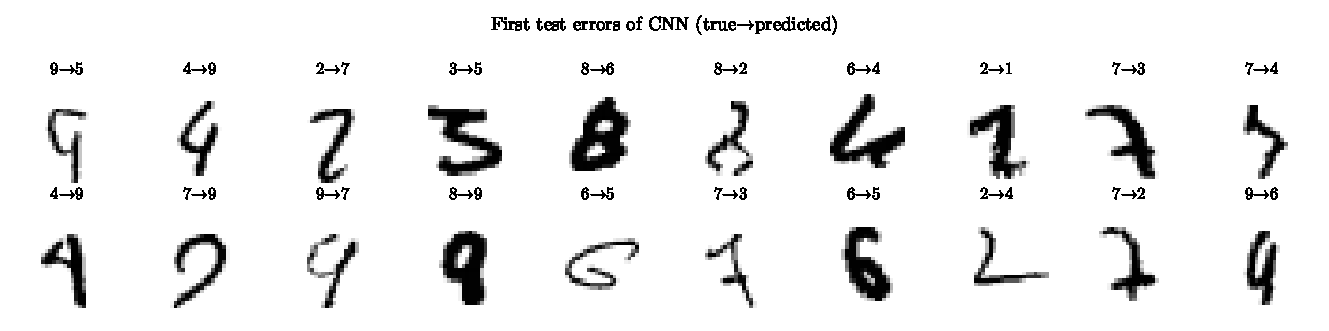
\includegraphics[width=\textwidth]{../results/figures/errors.pdf}
\caption{Hai mươi ảnh test đầu tiên MLP dự đoán sai (nhãn thật$\to$dự đoán).}
\label{fig:errors}
\end{figure}

\subsection{Giới hạn của kết quả}
\begin{itemize}
\item \textbf{Một seed.} Mỗi mô hình chính chỉ được huấn luyện một lần (seed 42) và chỉ có một phép chia train/validation. Riêng MLP chúng tôi có ba seed trong thí nghiệm tăng cường (\cref{tab:augmentation}): độ lệch chuẩn của test accuracy giữa các seed là cỡ vài phần mười điểm phần trăm, tức cùng bậc với chênh lệch giữa MLP và scikit-learn.
\item \textbf{Quét tuần tự.} Coordinate descent một vòng không xét tương tác giữa các siêu tham số (ví dụ learning rate tối ưu phụ thuộc kích thước batch và momentum) và có thể bỏ lỡ tổ hợp tốt hơn. Thứ tự quét cũng ảnh hưởng đến kết quả.
\item \textbf{Chọn trên validation, báo cáo trên test.} Test chỉ được dùng một lần cho mỗi cấu hình cuối cùng. Với Naïve Bayes, test cao hơn validation (\accTestNB\% so với \accValNB\%), điều thường thấy ở MNIST vì tập test chính thức dễ hơn một chút; chúng tôi không dùng điều này để chọn gì.
\item \textbf{Một máy, CPU, có nhiễu.} Thời gian đo trên một máy; không dùng GPU. Một số lượt chạy (các baseline scikit-learn, tuning) có thể trùng thời gian với công việc khác nên chỉ dùng để so bậc độ lớn.
\item \textbf{Phạm vi.} Kết quả chỉ nói về MNIST: ảnh $28\times28$, căn giữa, một chữ số. Bản demo web cắt, thu nhỏ và căn giữa nét vẽ theo cách của MNIST nhưng chữ viết trên màn hình vẫn khác phân phối huấn luyện, nên có thể sai ở những ca MLP không sai trên tập test.
\end{itemize}
